% Une ligne commentaire débute par le caractère « % »

\documentclass[a4paper]{article}

% Options possibles : 10pt, 11pt, 12pt (taille de la fonte)
%                     oneside, twoside (recto simple, recto-verso)
%                     draft, final (stade de développement)

\usepackage[utf8]{inputenc}   % LaTeX, comprends les accents !
\usepackage[T1]{fontenc}      % Police contenant les caractères français
\usepackage[francais]{babel}
\usepackage{hyperref}


\usepackage[a4paper,left=2cm,right=2cm]{geometry}% Format de la page, réduction des marges
\usepackage{graphicx}  % pour inclure des images

%\pagestyle{headings}        % Pour mettre des entêtes avec les titres
                              % des sections en haut de page

 \title{  Qui est-ce ?\\         % Les paramètres du titre : titre, auteur, date
  Projet de programmation}          
\author{Groupe \emph{Erasmus}\\
  \emph{Ali Mohammed, Alexander Goldberg et Eugène Ton}\\
  L2 informatique\\
  \emph{\url{https://github.com/Alex-Gberg/projet-erasmus}}\\
  Faculté des Sciences\\
Université de Montpellier.}
\date{\today}             


\begin{document}

\maketitle                    % Faire un titre utilisant les données
                              % passées à \title, \author et \date

\begin{figure}[ht]
    \centering
    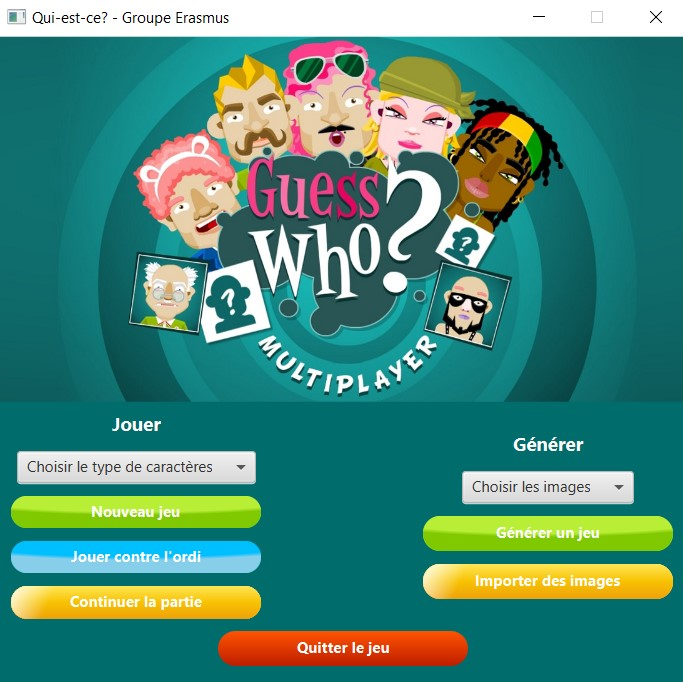
\includegraphics[width = 10cm, height=10cm]{qui est ce main menu.jpg}
    \caption{Menu principal}
\end{figure}
\newpage

\begin{abstract}     % Résumé du travail

  \emph{Description très succinte du problème et des différentes étapes de réalisation}

\end{abstract}


\section{ Technologies utilisées  et organisation} % Commencer une section, etc.


\subsection{Choix du langage}         % Section plus petite

Les langues utilisées dans ce projet de « Qui-est-ce » sont Java et JSON. La version 11+ de Java est demandée.\\
Les frameworks utilisés sont JSON et CSS, elles sont bien compatibles avec Java.
Le projet exige une utilisation de JSON pour le jeu « Qui-est-ce », cependant le parsing entre JSON et Java est bien documenté et pratiqué.\\
Nous utilisons la bibliothèque Javafx pour créer l’interface utilisateur et tout objet visible et interactif.\\
Le parsing de JSON au Java, est programmé avec l’aide de la bibliothèque Gson, développée par Google. Gson a été prouvé à être reliable par beaucoup d’utilisateurs, la documentation de Gson est aussi très large et utile pour tout utilisateur.\\
L’environnement de programmation utilisée est IntelliJ IDEA.



\subsection{Organisation du travail}

La répartition du travail avait été faite entre nous pendant nos sessions de travail en groupe. Nous avons utilisé les « issues » sur github pour se guider et répartir le travail, mais les « commits » et les « pushs » sur notre github ne sont pas précis, on a toujours planifié au moins 2 séances de travail en groupe par semaine ou on travaillait ensemble collectivement sur ce projet. Souvent, on effectuait des recherches plus complexes ensemble.\\

Après avoir complété et testé des tâches, on les présentait dans nos séances de travail en groupe et on s’envoyait le code entre nous. La majorité des « Commits » ont été faits par Alexander Goldberg qui est aussi le créateur du github.\\


Les fonctions principales des « issues » sur notre github sont:
\begin{itemize}
\item Informations sur l’état du projet et ce qui nous manque.
\item Laisser des commentaires pour le travail collectif.
\item Les « tags » et « milestones » servent aussi comme marqueur pour l’importance d’un « issue ».
\item Décomposition des tâches en plusieurs tâches plus petit.
\item Organisation propre pour un projet en groupe et facile à rattraper pendant nos séances de groupe.\\
\end{itemize}


Les « issues » peuvent aussi avoir une caractéristique, « Milestone », qui marque une tâche avec une étiquette. Des « Milestone » utilisés dans ce projet sont « Generator », « Game », « Extension » et « Report ». Chaque « Milestone » peut avoir une date limite, donc ça marque aussi la date limite de certains « issues ».
\newpage

\section{Étape 1 : permettre à l'utilisateur de jouer}


\begin{figure}[h!] 
  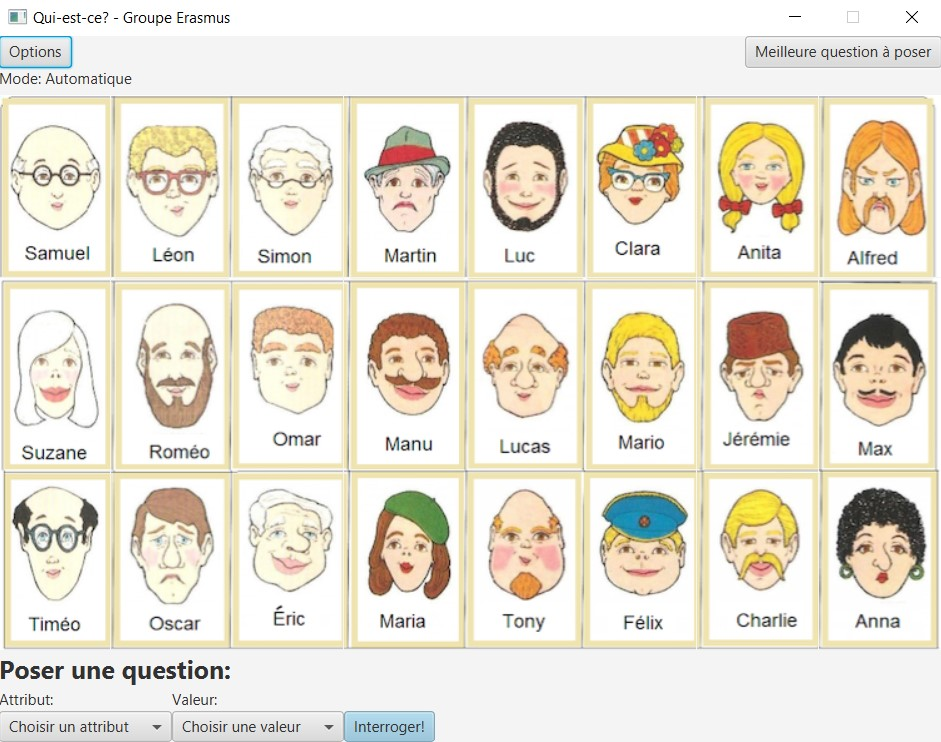
\includegraphics[width = 16cm, height=12cm]{normal game.jpg}
  \caption{« Qui-est-ce » classique}
\end{figure}


Lors de l’exécution de notre programme, l’utilisateur est accueilli par le menu ou avec plusieurs fonctionnalités. L’utilisateur peut choisir un ensemble d’images et le jouer, il peut aussi jouer une partie sauvegardée comme il peut aussi sauvegarder une partie non terminée.\\
Le jeu est en mode Automatique par défaut, ainsi les personnages non conformes à la réponse seront éliminés automatiquement. L’utilisateur peut changer le jeu au mode manuelle, où l’utilisateur reçoit les réponses à ses interrogations, mais il sera obligé d'éliminer les personnages manuellement en cliquant sur les images avec sa souris. Pendant la session de jeux, l’utilisateur peut changer le mode depuis le bouton « Options » en haut de la fenêtre. L’utilisateur a aussi la liberté de changer ce mode pendant la partie.\\

\begin{figure}[ht]
    \centering
  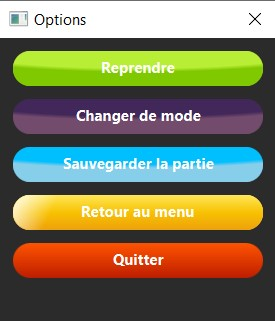
\includegraphics[scale=1]{normal game options.jpg}
  \caption{« Qui-est-ce » options}
\end{figure}

Le menu « Options » donne aussi accès au bouton « Sauvegarder la partie ». La sauvegarde d’une partie de « Qui-est-ce » est faite en modifiant le fichier de sauvegarde JSON, la continuation d’une partie sauvegardée est donc faite en lisant le fichier de sauvegarde JSON. Le programme n’a qu’un fichier de sauvegarde, donc si l’utilisateur sauvegarde une partie, l’ancienne partie sauvegardée est d’abord écrasée et ensuite remplacée par la nouvelle partie. Pour continuer le jeu que l’utilisateur a sauvegardé, l’utilisateur doit utiliser le bouton « Continuer la partie » depuis le menu principal.\\
Le menu d’options change dans certains cas, le menu d’option de base affiche les choix, « Reprendre », « Retour au menu » et « Quitter ». Pendant une session dans le mode de jeu, deux options s’y ajoute, « Changer de mode » et « Sauvegarder la partie ».\\


Le format de JSON est inspiré de la présentation d’introduction au projet de programmation.  Le format de JSON dans ce projet a en première ligne le « path », donc le chemin d’accès au dossier d’images. En deuxième et troisième ligne, il y a les dimensions de la grille. Le reste du fichier JSON consiste de plusieurs objets numérotés qui sont enregistrés dans l’objet « possibilities ». L’index des objets numérotés en « possibilities » représentent le nombre d'images dans l’ensemble d’images. Toutes les images ont tous les attributs communs de cet ensemble, mais des valeurs différentes. Les attributs et valeurs sont enregistrés sous l’index de l’image.\\
Le format du fichier de sauvegarde JSON prend 3 objets, le fichier JSON du jeu de base comme générateur, l’index de la cible et une liste du type boolean pour confirmer les caractères éliminés.\\
Cependant, notre format de JSON a des contraintes. D’abord, le chemin d’accès doit être un dossier contenant toutes les images du ensemble. Ensuite, la grille dans le jeu de « Qui-est-ce » doit être complète, donc la multiplication entre le nombre de colonnes et lignes doit être égale au nombre d’images. Finalement, les noms des fichiers images doivent être différents.\\

Les requêtes traitées apparaissent dans le menu principal et pendant une partie de jeu en mode automatique ou mode manuelle. Les attributs possibles et originels du jeu « Qui-est-ce » ont été recherchés sur internet. \\
Les attributs choisis pour le jeu de base « Qui-est-ce » sont : « Nom », « Genre », « Cheveux », « Lunettes », « Chauve », « Chapeau », « Cheveux longs », « Cheveux boucles », « Grande bouche », « Moustache », « Barbe », « Boucles oreilles ». Les valeurs à ces attributs sont soit « oui » ou « non ».\\

Pendant une partie, l’utilisateur est présenté avec deux menus déroulant dans le tableau de bord. Le premier menu déroulant est le sélecteur d’attributs, le deuxième menu déroulant est le sélecteur de valeurs. Le mode de jeu automatique ou manuelle n’affecte pas ces menus déroulants.\\

Le programme contient plusieurs classes et des structures de données pour la visualisation, le parsing et traitement de JSON à Java et des listes pour organiser les données physiques.\\
La librairie « Javafx » est bien adaptée à Java, elle possède de nombreuses documentation et extensions. Ce projet utilise principalement, des fenêtres, des boutons, des menus déroulants, des grilles d’images, des champs de textes.\\
La librairie « Gson » est connue pour le traitement et parsing des fichiers JSON à Java.
Des autres structures de données comme le « HashMap », « Node », « ArrayList », « ObservableList », « JsonObject » et « TreeMap » ont été utilisé comme aide pour le traitement des fichier JSON et données physiques tout au long du projet. L’utilisation de ces structures de données diverses dans leur classe respective, seront expliquées prochainement.\\

Voici les classes individuelles du jeu de base.
\begin{enumerate}
    \item      La classe « Main » lance le programme et lance le menu principal avec l’aide d’un « Stage ».\\
    
    \item      La classe « Menu » est le moteur du menu principal et la fenêtre du menu principal. Les actions des évènements « Stage « Button » et « ComboBox » (menu déroulant) du menu principal sont défini ici. Les fonctions d’aide telles que, vérifier que les types du dossier choisi n’a que des images, vérifier que le dossier choisi a au moins un image et sauvegarde du répertoire y sont inclus.\\
    Les structures de données à noter ici sont :
    \begin{itemize}
        \item « ObservableList<String> » imageSets, il permet de retourner les noms des dossiers d’images, afin de les afficher dans le menu déroulant.
        \item « ArrayList<String> playableGames » qui retourne la liste d’ensemble de caractères afin de les afficher dans le menu déroulant.
        \item « DirectoryChooser dc = new DirectoryChooser() » pour sélectionner un dossier manuellement dans l’explorateur de l’utilisateur.\\
    \end{itemize}
 
    \item      La classe « Display » est responsable pour tout traitement d’image.\\
    Le premier constructeur de Display lit un fichier JSON et peut créer une grille avec les caractères avec les informations du fichier JSON, le deuxième constructeur peut créer une grille basée sur un dossier d’images.\\
    Le moteur de Display contient plusieurs fonctions tels que, charger des images basés sur un fichier JSON ou un dossier d’images et les ajouter à la liste d’images, barrer des images basés sur son index qui est mieux adapté pour le mode de jeu automatique, barrer des images basés sur l’image lui-même qui est mieux adapté pour le mode de jeu manuel, barrer un image visuellement à l’aide de la librairie « javafx.scene.Group » qui peut recouvrir un image sur l’autre et recevoir un image seul, y sont inclus.\\
    
    Les structures de données à noter ici sont :
    
    \begin{itemize}
        \item L’« ArrayList<Node> », il contient toutes les images sous les types de « ImageView » et « Group », cette liste est donc utilisée pour ajouter des images, charger des images et visualiser des croix rouges au-dessus d'une image.
        \item Le « JsonElement » et principalement son extension « JsonObject », « JsonObject » est une classe représentant un type d'objet dans JSON.\\
        Un objet dans JSON se compose de paires nom-valeur où les noms sont des Strings et les valeurs sont tout autre type de « JsonElement ». Cela permet de créer une liste de « JsonElements ». Les éléments membres de cet objet sont conservés dans l'ordre dans lequel ils ont été ajoutés.\\
        La méthode « getAsJsonObject(‘’ String ‘’) » est pratique pour obtenir le membre spécifié en tant que JsonObject.\\
    \end{itemize}
 

 
    \item      La classe « Game » est le moteur et la fenêtre du mode de jeu.\\
    Les actions des évènements « Stage », « Button », « ComboBox » (menu déroulant) et « BorderPane » de la fenêtre du mode de jeu sont définies ici.
    Les fonctions d’aide tels que, proposer les attributs possibles dans le premier menu déroulant, proposer les valeurs possibles pour chaque attribut dans le deuxième menu déroulant, procès de la question, réponse sur la question choisie, barrer les images automatiquement ou manuellement à l’aide de la classe « Display », vérification si le nom choisi est la cible correcte et lancement de la fenêtre de congratulation, y sont inclus.\\
    A l’exception des structures de données primitives, les structures de données importantes à expliquer ici sont :
    \begin{itemize}
        \item « JsonObject » comme expliqué auparavant, cette structure de donnée est principalement utilisée pour accéder aux objets de JSON comme « possibilites », l’index (par exemple « 7 ») et n’importe quel autre objet (par exemple « fichier » ou « nom »).
        \item  « ArrayList<Boolean> crossedOut », cette structure de données est une liste booléenne pour savoir quel caractère est barré. Ceci nous aide à actualiser la grille pendant la session de l’utilisateur.
        \item « HashMap<String, Set<String>> propertyMap », cette structure de donnée permet d’utiliser un ensemble d’attribut comme clés pour une meilleure compatibilité avec des fonctions comme par exemple, « setItems() » de « ComboBox ». Le format de JSON est d’abord séparé en chaque attribut, ces attributs individus sont traités comme clés, ensuite elles sont ajoutées à une « HashMap », finalement la « HashMap » est retournée. Ceci est important pour attribuer plusieurs valeurs à un attribut et afficher toutes les options dans les menus déroulant.\\
    \end{itemize}
 


    \item      La classe « Options » est le moteur et la fenêtre du bouton « Options » qui est affiché à chaque instance du jeu.\\
    Les actions des évènements « Stage », « Button » et « BorderPane » de la fenêtre d’options sont définies ici. Les fonctions d’aide tels que, choix d’options de base (« Reprendre », « Retour au menu » et « Quitter ») et choix d’options supplémentaires (« Changer de mode » et « Sauvegarder la partie »), y sont inclus.\\
    Il faut noter que les options de bases sont retenues dans la fonction « setDefaultOptions() » et les options supplémentaires pour le mode de jeu sont retenues dans la fonction « setGameOptions() ».\\
    
    \item La classe « Save » permet de créer et sauvegarder un nouveau fichier JSON.\\
    La structure de donnée, ArrayList<Boolean> crossedOut, sert à sauver les caractères éliminés afin de les barrer de nouveau lors d’une continuation de cette partie. Cette liste est importante pour toute opération qui nécessite une liste de charactère éliminé.\\
    La classe « Save » est en outre responsable pour la sauvegarde d’une partie, on peut dire que « Save » est le générateur du fichier de sauvegarde.\\
    
    \item La classe « Congratulations » contient la fenêtre de congratulations qui est lancée lors d’une victoire. Elle affiche deux boutons « Play Again », « Quit » et un GIF pour féliciter l’utilisateur de son succès.\\
    \begin{figure}[h!]
        \centering
        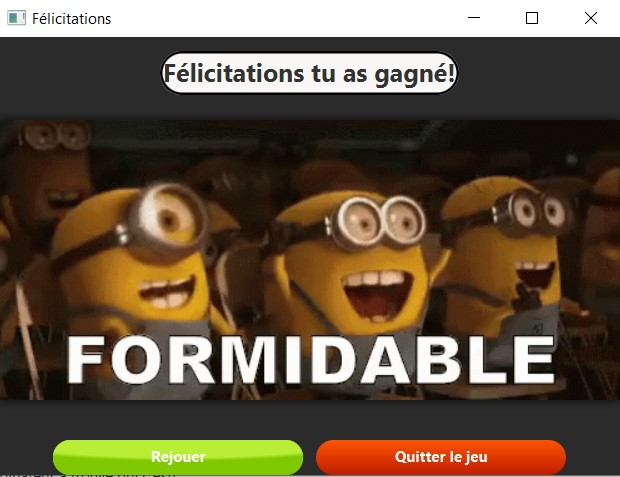
\includegraphics[width= 6cm, height=4cm]{win scene.jpg}
        \caption{Félicitations}
    \end{figure}
    
\end{enumerate}
Dans une partie en mode manuelle, le programme vérifie si la personne cible est en fait touchée par la question, la réponse est ensuite affichée dans l’interface, l'utilisateur a la possibilité de rayer n’importe quel caractère avec un simple clic sur le caractère affiché sur la grille.
Dans une partie automatique, le programme vérifie aussi si la personne cible est en fait touchée par la question, la réponse est ensuite affichée dans l’interface, mais après le programme passe par tous les autres caractères affichés et non rayés, afin de rayer automatiquement tous les caractères avec une réponse négative.
Si la correcte cible a été choisie, la fenêtre de « Congratulations » apparaît, l’utilisateur a ensuite le choix de continuer à jouer ou bien d'arrêter à jouer.



\section{Étape 2 : aider  à la saisie  des personnages}

\begin{figure}[ht]
    \centering
    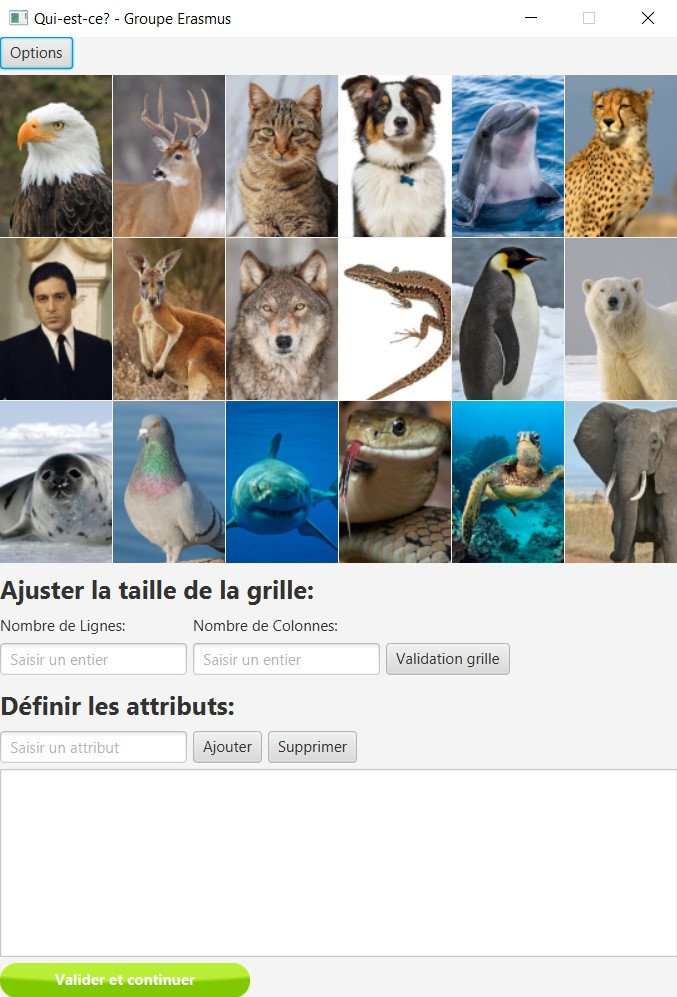
\includegraphics[width= 10cm, height=12cm]{generator game.jpg}
    \caption{Génération d'un fichier JSON sur des animaux}
\end{figure}

Etant donné un ensemble d'images, si nous voulons créer un jeu jouable, nous devons le programmer en dur, donc il faut écrire un fichier JSON adapté à notre format en dur. Cette contrainte peut être levée en créant un mode de générateur pour l’utilisateur. L’utilisateur aurait alors le choix de créer son propre fichier JSON basé sur un type d’ensemble d’images. La saisie pour l’ensemble d’images est un dossier d’images dans le bon répertoire (« "src/main/resources/character\_sets/" »), et le résultat de ce mode générateur est un fichier JSON crée par l’utilisateur en accordant des attributs et valeurs à un ensemble d’images.\\

La classe « Generator » est le moteur du mode générateur et la fenêtre du mode générateur. Les actions des évènements « Stage », « Button », « ComboBox » (menu déroulant) et « BorderPane » de la fenêtre Generator sont définies ici. Les fonctions d’aide tels que, redimensionner la grille, saisie et création de la liste d’attribut, nomination de chaque image, vérification que chaque image a un nom unique, saisie de valeurs à tous les caractères, vérification que chaque image a un ensemble de valeur unique, allocation des valeurs aux caractères après vérification, sauvegarde des valeurs dans une liste de possibilité qui contient tous les informations sur les caractères, nomination et sauvegarde du fichier de JSON, y sont inclus.\\
Avec l’aide de la structure de donnée « Node », les entrées d’attributs et valeurs sont représentées dans une liste d'objets.\\

Lors d’un ajout d’attribut, le texte entré dans le champ de texte « TextField attributeInput » est d’abord modifié en casse basse par la méthode « String » prédéfinie « toLowerCase() ». Ensuite, le code vérifie si le texte n’est pas vide en la comparant avec « 0 », n’est pas déjà contenu dans la liste d’attribut avec « !attributeList.contains(text) », n’est pas « nom » ou « fichier ». Finalement, le texte vérifié est ajouté à la liste d’attribut du code « ObservableList<String> attributeList » et dans la liste visuelle « ListView<String> attributeListView ». Au cas échéant de la vérification, le champ de texte est vidé et le texte n’est pas ajouté à la liste d’attributs. Lors de la suppression d’un attribut, le code supprime l’attribut sélectionné dans la liste visuelle « attributeListView » par la méthode prédéfinie « remove() » de « ObservableList<String> », la sélection est exécuté avec « attributeListView.getSelectionModel().getSelectedItem() ». Une fois tous les attributs entrés, l’utilisateur peut passer à la définition d’attribut pour chaque image. Lors de la définition d’attribut, l’image en question est affichée avec \\« singleImageDisplayVbox.getChildren().setAll(display.getSingleImage(currentImageIndex)); ».\\
Le code définit la structure de donnée des valeurs choisie pour les attribtus avec « HashMap<String,TextField> textFieldMap = new HashMap<>(); ».\\
Le champ de texte « nom » et toutes les valeurs sont obligatoires pour toutes les images. Le nombre de valeurs exigé est inconnu par le code, donc le code exécute une boucle « for (String attribute : attributeList) » avec « textFieldMap.put(attribute, new TextField()); » comme instruction, afin de créer un champ de texte pour chaque attribut.\\
Lors de la validation des valeurs du dernier image, le code passe par tous les attributs avec une boucle « for (String attribute : attributeList) », il vérifie si tous les attributs ont été défini avec « if(userInput.length() == 0) » comme instruction.\\ Avec des méthodes auxiliaires, il vérifie si tous les images ont un nom différent en exécutant « if (possibilites.get(String.valueOf(i)).get("nom").equals(possibilites.get(String.valueOf(j)).get("nom"))) » et si tous les images ont un ensemble de valeurs différent par « if(iAttributes.equals(jAttributes)) », où « iAttributes » et jAttributes » représentent deux différents ensembles de valeurs à la fois pour la comparaison.\\
Les valeurs valides sont ensuite ajoutées à « TreeMap<String,HashMap<String, String>> possibilities; », qui contient toutes les valeurs possibles dans une « Map » de Java.\\
Ensuite, l’utilisateur doit nommer le fichier JSON, le code vérifie que le nom saisi soit pas vide et surtout qu’il n’aie pas de caractères illégaux comme :
\begin{center}
 « "/", "\textbackslash n", "\textbackslash r", "\textbackslash t", "\textbackslash 0", "\textbackslash f", "`", "?", "*", "\textbackslash \textbackslash", "<", ">", "|", "\textbackslash", ":" »\\
\end{center}

La vérification de caractère illégaux est fait avec l’aide de la structure de donnée « CharSequence[] ILLEGAL\_CHARACTERS », qui contient tous ces caractères, le code exécute une boucle « for(CharSequence c : ILLEGAL\_CHARACTERS) » qui passe par la liste et crée une alarme si le nom contient un des caractères par « if (proposedName.contains(c)) » comme instruction. Après le nommage de fichier JSON, la création du fichier JSON est réussie, l’utilisateur peut choisir de jouer au nouveau jeu de « Qui-est-ce », retourner au menu principal ou bien quitter l’application.\\

C’est important à noter que la classe Display a été programmé avec des constructeurs polymorphes, tout ce qui concerne la classe du générateur est à l'intérieur de la classe Display. Des structures de données Java, notamment HashMap, sont utilisées pour la création d’un fichier JSON avec des clés. Il faut que passer un HashMap à gson.toJson() et il créera automatiquement un fichier JSON en respectant les clés. Donc, la création des HashMap est faite dans le générateur afin qu'ils soit traité lorsqu’il est passé à la fonction gson.toJson(). La classe « GeneratorCompletion » contient le moteur et la fenêtre de congratulation lors d’une création d’un fichier JSON réussie.\\

Forcément, quelques implémentations au programme de base ont été faites pour optimiser l’expérience de l’utilisateur.\\
Le menu principal est divisé en deux parties, gauche pour le mode de jeu et droite pour le mode générateur.\\
Pour le mode de générateur, l’utilisateur est présenté avec un menu déroulant (« Choisir les images ») pour choisir un des dossiers d’images déjà présent au répertoire, un button pour le lancement d’une session en mode générateur (« Générer un jeu ») et un dernier bouton pour importer son propre dossier d’images avec des images personnalisés (« Importer des images »).\\
Avant de générer un jeu, il faut choisir un dossier d’images du menu déroulant, l’utilisateur a alors le choix entre un dossier d’image déjà présent dans le menu déroulant ou bien il importe son propre dossier d’image. Lorsque l’utilisateur appuie sur « Importer des images », il est présenté avec son propre explorateur pour choisir le dossier d’image. Après avoir importé un dossier d’image, il peut le retrouver sous le nom respectif dans le menu déroulant. Finalement, l'utilisateur peut lancer le mode générateur.\\
L’utilisateur peut modifier les dimensions de la grille d’images présentée en saisissant et validant les nombres de lignes et colonnes souhaité dans les deux champs de textes en dessous de la section « Ajuster la taille de la grille ».\\
Sous la section « Définir les attributs », l’utilisateur peut saisir un attribut dans le champ de texte et l’ajouter à la liste d’attribut en appuyant sur le bouton « Ajouter ».\\
L’utilisateur peut supprimer des attributs en les sélectionnant manuellement dans la liste d’attribut en dessous et appuyant le bouton « Supprimer ».\\
Après avoir saisi les attributs communs souhaités, l’utilisateur doit valider la liste d’attribut avec le bouton « Valider ».\\
Ensuite, le générateur passe aux valeurs des attributs, le générateur présente l’utilisateur avec tous les images individuellement l’un après l’autre.\\
Si toutes les images ont été nommées et remplies, le générateur affiche un dernier champ de texte pour le nom du fichier JSON, ce nom sera le nom d’affichage dans le menu déroulant pour le mode de jeu « Qui-est-ce ».\\
En cas ou l’utilisateur essaie de valider un nom de fichier contenant un de ces caractères spéciaux, le générateur notifie l’utilisateur que ces caractères spéciaux ne sont pas acceptés et la validation est rejetée.\\
La validation du nom de fichier JSON met fin au mode générateur. Le fichier JSON ne peut plus être modifié automatiquement par le programme.\\
Après la validation et vérification du nom de fichier, l’utilisateur est présenté avec une fenêtre avec deux boutons qui propose de jouer une partie de « Qui-est-ce » avec le nouveau fichier JSON tout de suite ou bien retourner au menu. Le fichier JSON se trouve maintenant dans le répertoire des ressources JSON. Donc il est sélectionnable dans le menu déroulant pour démarrer une partie de « Qui-est-ce ».
\newpage


\section{Étape 3 : Extension, mode contre ordinateur}

\begin{figure}[ht]
    \centering
    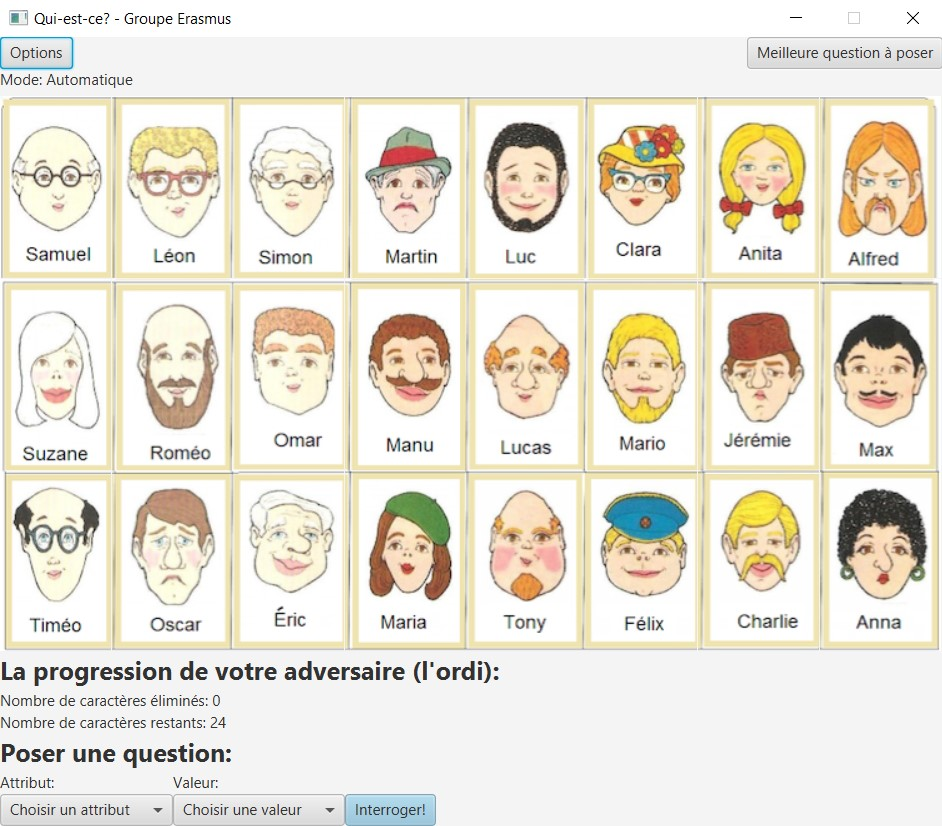
\includegraphics[width= 16cm, height=14cm]{game vs bot.jpg}
    \caption{« Qui-est-ce » contre l'ordinateur}
\end{figure}


Voici les extensions réalisées pour le jeu de « Qui-est-ce ».\\
L’extension principale est un jeu de « Qui-est-ce » contre l’ordinateur. L’utilisateur peut jouer n’importe quel jeu de « Qui-est-ce » contre l’ordinateur, il peut aussi sauvegarder et reprendre une session de « Qui-est-ce » contre l’ordinateur. En addition à cette extension, un bouton de triche pour l’utilisateur a aussi été réalisé. Ce bouton est toujours disponible pendant n’importe quelle session de « Qui-est-ce ».\\

Cependant, plusieurs décisions ont été prises pour le développement des extensions.\\
L’algorithme de l’ordinateur choisi assure la meilleure question/ requête à poser, il essaie toujours d' éliminer la moitié plus ou moins. L’algorithme parcourt toutes les valeurs des caractères restants et cherche la fréquence de la valeur la plus proche de la moitié du nombre de caractères. La valeur correspondante est ensuite la requête utilisée par l’ordinateur.\\
Le bouton de triche pour l’utilisateur, utilise l’algorithme de l’ordinateur avec les caractères restants de l’utilisateur. Ce bouton affiche seulement un texte indiquant la meilleure requête. Cela permet à l’utilisateur de simplement comparer les requêtes. Ce bouton n’est pas un mode de triche, le bouton indique la meilleure requête à poser au moment appuyé. Si l’utilisateur souhaite tricher plus qu’une fois, il doit réappuyer sur le bouton de triche afin d’aggraver sa honte.\\
Dans cette extension, l’utilisateur et l’ordinateur ont la même cible et les deux joueurs ne savent pas qui est la cible. Donc c’est important de cacher la grille de caractères de l’ordinateur, l’utilisateur pourrait tricher en analysant la grille de l’ordinateur. Cependant, l’utilisateur est présenté avec une section de texte indiquant le nombre de caractères éliminé et restant de l’ordinateur.\\
Si l’ordinateur trouve la cible d’abord, alors la section de texte de l'ordinateur affiche que l’ordinateur a trouvé la cible et il a gagné. Mais le jeu de « Qui-est-ce » contre l’ordinateur ne peut qu’être terminé par l’utilisateur, il peut terminer le jeu en requêtant la cible et passer ensuite à la fenêtre de félicitations, ou il peut fermer l’application par force. Ce choix a été pris, puisque certains joueurs souhaitent chercher la cible même si l’ordinateur l’a déjà trouvé. Donc, pour certains, ce jeu peut sembler comme un jeu de « Qui-est-ce » régulier qui se joue en parallèle avec un ordinateur.\\
Le jeu de « Qui-est-ce » contre l’ordinateur peut être sauvegardé, la session sauvegarde aussi la progression de l’ordinateur, cette session peut être reprise en mode « contre l’ordinateur ». Donc la continuation de cette session sera contre le même ordinateur. Cependant, une session de « Qui-est-ce » classique sauvegardé peut aussi être reprise en mode classique.\\
D’ailleurs, le mode automatique ou manuelle n'affecte pas l’algorithme ou la performance de l’ordinateur. L’algorithme de l’ordinateur prend les données de la liste « crossedOut », elle est indépendante du mode automatique ou manuelle.\\
Continuons, avec la description de la résolution, cela contient des explications précises sur le code de l’ordinateur. Les protocoles, algorithmes et les objets visuelles sur l’ordinateur sont expliqués en détail avec des bouts de code.\\





La classe « Bot » contient les caractéristiques du bot, le processus de choix du bot, les messages des requêtes au terminal et la mise à jour des caractères eliminé. L’algorithme de choix de requête du bot est dans la classe « GameUtils », elle sera expliquée prochainement.\\

Le code de la classe « Bot » commence par déclarer cinq variables globales : « jsonRoot », « target », « crossedOut », « numPics » et « found ». « jsonRoot «  représente un objet JSON, « target » représente la cible du jeu, « crossedOut » représente la liste de caractère eliminé, « numPics » représente le nombre de caractère dans le jeu joué et « found » est une valeur booléenne qui représente si le bot a trouvé la cible. Il faut noter que « final JsonObject jsonRoot; » et « ArrayList<Boolean> crossedOut; » sont deux structures de données complexes. Le constructeur est l'endroit où les valeurs de ces variables sont définies.\\

La méthode « playTurn » commence par une instruction if qui vérifie si « found » est faux. Si « found » est faux, alors le code crée une ArrayList d'objets String par « ArrayList<String> qToAsk », elle représente la question à demander par le bot. De plus, le code appelle la méthode « algoChoice » de la classe « GameUtils » pour choisir la requête la plus efficace. « qToAsk » contient un attribut et une valeur correspondante.\\
Le code parcourt ensuite la liste, si le premier élément de la liste est égal à « nom », alors « found » est modifié à « true » et un message s'affiche dans le terminal indiquant « Bot : Found -> "x" ».\\
Le bot choisit qu’un « nom » s’il a trouvé sa cible, donc « qToAsk » contient « nom » comme attribut si et seulement si le bot a trouvé la cible.\\
Sinon, le code appelle la fonction « processGuess(qToAsk.get(0),qToAsk.get(1)) » avec tel paramètre.\\
Si « found » est « true » dès le début, alors nous savons que le bot a déjà trouvé la cible, donc il faut attendre que l’utilisateur trouve la cible ou bien ferme le jeu par force.\\

La méthode « processGuess » prend deux Strings comme paramètre, ces Strings représentent un attribut et une valeur correspondante. En outre, une requête dans le jeu. Le code de cette méthode consiste à procéder une requête du bot, en comparant la requête choisie avec les valeurs de la cible, le code affiche une phrase dans le terminal indiquant la requête précise et le résultat. De plus, cette méthode met à jour la liste de caractère éliminé du bot.\\
Le code commence par définir « JsonObject pers = jsonRoot.getAsJsonObject("possibilites"); » et « boolean response = value.equals(pers.getAsJsonObject(String.valueOf(target)).get(property).getAsString()); ».\\
Le « jsonRoot » est un nœud racine qui contient toutes les valeurs possibles pour cet objet JSON. Il obtient ensuite les possibilités en tant que « JsonObject », qui est un objet avec des attributs et des valeurs.\\
Le « response » est une valeur booléenne qui représente l’égalité de la valeur de la requête du bot et la valeur de la cible. Donc, si la requête correspond à la valeur de la cible, « response » sera « true ».\\

Après cela, la mise à jour de la liste « crossedOut » est éxecuté. Il y a deux boucles : la boucle extérieure parcourt toutes les images de « numPics » par « for (int i = 0; i < numPics; i++) » et la deuxième boucle intérieure « if(!crossedOut.get(i)) » qui s’éxecute si l’image à la position « i » n’est pas dans la liste « crossedOut ». La boucle intérieure, contrôle si l’image à la position « i » est conforme à la requête, si elle est conforme, alors rien ne ce passe. Par contre, si elle n’est pas conforme, elle est ajoutée à la liste « crossedOut » et éliminée des requêtes futures du bot.\\
Le contrôle dans la boucle intérieure est fait en comparant la valeur booléenne « response » à une nouvelle valeur booléenne qui représente l’égalité de la valeur de l’image à la position « i » et la valeur de la requête, tel que « value.equals(pers.getAsJsonObject(String.valueOf(i)).get(property).getAsString()) ». Une image doit être éliminée si sa valeur ne conforme pas au résultat de la requête du bot. Donc, si les deux valeurs booléennes sont différentes, l’image doit être éliminée car elle ne conforme pas à la requête du bot.\\
Dans la boucle intérieure, deux boucles « if » sont utilisées pour chaque cas ou les valeurs seraient différentes, tel que « if (!response \&\& value.equals(…) » et « else if (response \&\& !value.equals(…) ».\\

La classe de « Bot » contient « VBox getBotInfo() », qui affiche les informations du bot. Dans le jeu contre l'ordi (le bot), le jeu affiche le nombre de caractère éliminé et restantes dans des « Label » dans la « VBox ». Les informations sont mises à jour après chaque requête du bot, le code calcule le nombre éliminé en comptant les valeurs vraies dans la liste de « crossedOut » par «int numCrossedOut = GameUtils.numTrue(crossedOut) ». Le nombre de caractères restant est donc la soustraction du nombre d’images et le nombre d’images éliminé, le code exécute « (int numRemaining = numPics \- numCrossedOut) ». Si, le bot a trouvé la cible, alors les « Label » sont remplacés par un « Label » indiquant « L'ordinateur a trouvé qui c'est! ».\\

Finalement, la classe « Bot » contient deux méthodes « getteur », l’un retourne la liste booléenne « crossedOut » qui contient la liste d’images éliminées. L’autre retourne la valeur booléenne « found » qui est seulement vraie si le bot a trouvé la cible.\\
 
L’algorithme de choix de requête du bot se trouve dans la classe « GameUtils », elle contient des fonctions auxiliaires de la classe « Game ». Le code sous ci-dessous explique l’algorithme de choix le plus efficace pour n’importe quel jeu de « Qui-est-ce ».\\
Le code commence par déclarer un HashMap de ArrayLists. La clé est le nom d'un attribut et la valeur est un nombre entier qui représente le nombre d’apparition dans le texte.\\
Le code continue à déclarer une autre variable tel que « int remaining = crossedOut.size() - numTrue(crossedOut) ;», elle représente le nombre d’image non éliminé. La liste «crossedOut » contient des valeurs booléennes pour chaque image, donc « crossedOut.size() » retourne le nombre d'images. L’initialisation de la variable « remaining » soustrait du total d’images, le nombre de fois où chaque élément a été trouvé vrai par la fonction « numTrue() », ce qui nous donne le nombre de restes.\\

Expliquons la méthode « numTrue(ArrayList<Boolean> boolArray) » avant de continuer avec « algoChoice() », elle compte toutes les valeurs booléennes vraies dans une liste booléenne. En première ligne, le code initialise une variable compteur tel que « int count = 0; ». Ensuite, le code compte les valeurs vrais dans la liste avec une boucle « for (Boolean b : boolArray) » et son instruction « if (b) {count++;} ». Finalement, cette méthode retourne le nombre compté.\\

Continuons avec la méthode « algoChoice() », en préliminaire le code contrôle d’abord s'il n'y a qu'un seul image restante avec « if (remaining == 1) », dans ce cas la dernière vérification a réussi et le code renvoie une liste contenant juste « nom ». Sinon, le code continue par l’algorithme de choix de requêtes.\\
Ensuite, pour le choix de requête, l’algorithme assure toujours le meilleur choix de requête pour le bot. L'algorithme essaie de réduire le nombre de caractères restants par sa moitié au plus proche.\\ Le code calcule d’abord la moitié du nombre total d’images restantes avec « double half = remaining / 2.0 » et défini « double bestDistance = Double.MAX\_VALUE », qui représente la valeur maximale du type « double ». Le résultat de cette méthode est retourné en format d’une liste, donc le code initialise la liste « ArrayList<String> result = new ArrayList<>(); ».\\
La boucle « for (ArrayList<String> key : attributeFrequency.keySet()) » passe par tous les clés dans la liste d’attributs et valeurs. La boucle prend « if (Math.abs(attributeFrequency.get(key) - half) < bestDistance) » comme instruction afin de trouver la meilleure distance des valeurs fréquentes. Si, la boucle « if » est vrai, alors la valeur de « bestDistance » est mise à la nouvelle valeur « Math.abs(attributeFrequency.get(key) – half » et « result » prend la nouvelle clé (« key ») comme valeur.\\
Avec cette boucle, le code cherche la valeur absolue la plus proche de 0 afin de trouver la requête qui permet à réduire le nombre d’images restantes de moitié au plus proche, jusqu’à ce que la dernière image restante est trouvée. Le code utilise des valeurs du type « double » pour une meilleure précision lors des calculs, cela empêche des requêtes moins effectives.\\

En résumé, le code calcule une valeur absolue de la soustraction entre la fréquence d’une valeur quelconque et la moitié des images restantes, cela permet au code de comparer cette valeur absolue avec la variable « bestDistance » qui contient toujours la dernière valeur absolue la plus proche de 0. La comparaison est exécutée en boucle pour parcourir toutes les valeurs afin de trouver la meilleure distance, en d'autres termes, la valeur absolue la plus proche de 0. La clé de la valeur est ensuite ajoutée à la liste « result » qui contient la requête choisie. Finalement, la liste « result » est retournée.\\
 
La classe « Game » est responsable du lancement de jeu « Qui-est-ce », le code a deux constructeurs pour lancer le jeu. Un constructeur, « public Game(Stage stage, String jsonName, boolean vsComputer) » permet de lancer un jeu de « Qui-est-ce » contre le bot ou bien solo. L’autre constructeur « public Game(Stage stage, String jsonName, int target, ArrayList<Boolean> playerCrossedOut, boolean vsComputer, boolean compFound, ArrayList<Boolean> compCrossedOut) » permet de continuer un jeu de « Qui-est-ce » sauvegardée.\\
Le jeu sauvegardé peut être une session contre le bot ou bien solo. Le constructeur pour un jeu sauvegardé prend 4 paramètres de plus, la cible, la liste de caractère éliminé de l’utilisateur, la liste de caractère éliminé du bot et une valeur booléenne qui représente si le caractère a été trouvé par le bot.\\

Les deux constructeurs exécutent une condition pour déterminer si le jeu de « Qui-est-ce » est en mode contre l'ordi, « if (vsComputer) ». Le paramètre « vsComputer » est une valeur booléenne qui est mise à « true » lors du choix d’un jeu en mode contre le bot.\\
Le constructeur du lancement du mode de jeu exécute « this.bot = new Bot(jsonRoot, target, false, new ArrayList<>(crossedOut)); » pour initialiser le bot et créer le « VBox » dédié aux informations du Bot par « botInfo.getChildren().setAll(bot.getBotInfo() ».\\
Le constructeur de la continuation d’un jeu contre le bot exécute « bot = new Bot(jsonRoot, target, compFound, compCrossedOut) » pour initialiser le bot et crée le « VBox » dédié aux informations du Bot par « botInfo.getChildren().setAll(bot.getBotInfo() ».\\
Les deux constructeurs exécutent en première ligne « auxConstructor(stage, jsonName, vsComputer); », cela appelle à la méthode privé « auxConstructor(Stage stage, String jsonName, boolean vsComputer) » qui est un constructeur auxilliaire. Celui-ci crée l’affichage du jeu avec l’aide de la classe « Display » et « Options », de plus le bouton « Meilleure question à poser » est créé.\\

Le bouton « Meilleure question à poser » permet à l’utilisateur de tricher et elle est toujours disponible. Une fois appuyé, le bouton affiche en dessous du bouton un texte indiquant la meilleure question/ requête à poser en ce moment.\\
L'événement du bouton appuyé, exécute le code suivant :\\ « ArrayList<String> res = GameUtils.algoChoice(GameUtils.getAttributeFrequency(jsonRoot, crossedOut), crossedOut, jsonRoot) », ce code utilise la méthode « algochoice() » pour trouver la meilleure question à poser.\\
Ensuite, le code charge le texte dans un « Label » en dessous du bouton par « solvingAlgorithmLabel.setText( "Attribut: " + res.get(0) + ", valeur: " + res.get(1)) ». La position 0 de la liste « res » contient l’attribut, la position 1 de la liste contient la valeur. Finalement le tout est affiché. Le bouton de triche affiche toujours le choix du bot, qui est aussi optimal.\\

Voici un scénario d’interactions avec l’utilisateur:\\
L’utilisateur démarre l’application « Qui-est-ce », il décide de jouer une partie de « Qui-est-ce » contre l’ordinateur. L’utilisateur choisit le type de caractères « animaux » dans le menu déroulant sous la section de « Jouer ». Désormais, l’utilisateur appuie sur le bouton bleu « Jouer contre l’ordi ».\\

Le jeu commence et la fenêtre du jeu s’affiche. L’utilisateur est présenté avec une grille contenant tous les images/ caractères dans le jeu, un bouton d’options, un bouton de triche, un texte indiquant le mode de jeu, une section pour les informations du bot et une section pour le choix de l’utilisateur. L’utilisateur fier accepte le défi à jouer contre l’ordinateur en mode automatique.\\

Après une analyse des caractères et des valeurs, Il évite le bouton de triche et choisit l’attribut « canin » avec la valeur « Oui ». Le jeu affiche « Non » au-dessus du bouton « Interroger ! », l’utilisateur a éliminé 2 caractères, il lui reste 16 caractères. L’ordi a éliminé 9 caractères avec son algorithme de requête, il lui reste 9 caractères.\\

L’utilisateur continue par une deuxième requête, il choisit l’attribut « aile » et la valeur « Oui ». Le jeu répond par « Non », l’utilisateur a éliminé 3 caractères, il lui en reste 13. L’ordi a éliminé 4 caractères, il lui en reste 5.\\

L’utilisateur devient anxieux, il appuie discrètement sur le bouton de triche « Meilleure question à poser ». Le jeu affiche en dessous du bouton de triche un texte indiquant la requête, « Attribut : nombre de pattes, valeur :  4 », l’utilisateur valide la requête et le jeu répond par « Non ». L’utilisateur regagne de la confiance, il a éliminé 7 caractères, il lui reste 6 caractères. L’ordi a éliminé encore 2 caractères, il lui reste 3 caractères.\\

L’utilisateur continue à tricher, cette fois le jeu lui propose la requête « Attribut : habitat, valeur :  océan ». Après avoir validé la requête proposée, le jeu répond par « Non ». L’utilisateur a encore 4 caractères restant, l’ordi n’a qu’un caractère restant. Donc l’ordi doit encore choisir le nom de la cible.\\

L’utilisateur tend à son dernier recours, il essaie de deviner la cible, il a 1 chance sur 4. L’utilisateur se décide sur le kangourou, donc il valide l’attribut « nom » et la valeur « kangourou ». L’utilisateur a eu de la chance, son pari a été correct. Mais l’ordi a aussi trouvé la cible, donc cette partie a été un match nul. Néanmoins, l’utilisateur est présenté avec une nouvelle fenêtre contextuelle « Félicitations », cette fenêtre affiche un texte « Félicitations tu as gagné ! » et un GIF félicitant l’utilisateur de sa victoire. La fenêtre contextuelle affiche deux boutons, « Rejouer » et « Quitter le jeu ». « Rejouer » permet à l’utilisateur de retourner au menu principal, « Quitter le jeu » permet à l’utilisateur d’éteindre l’application.\\

L’utilisateur excité procède par appuyer sur le bouton « Rejouer » afin de gagner une partie contre l’ordi.



\section{Bilan et Conclusions}

Voici le bilan de ce projet de programmation, les fonctionnalités réalisées et non réalisées sont expliquées ici.\\

Toutes les fonctionnalités requises pour la première partie (jeu de « qui-est-ce » générique), ont été réalisées, sauf l’option de requêtes complexes. Les requêtes complexes sont des requêtes à multiples questions séparées par les opérateurs « et/ ou ». Cependant, le projet est capable de prendre en entrée un descriptif du jeu en format JSON, à permettre de poser des questions simples, à gérer les décisions graphiquement, sauvegarder ou reprendre une partie et finalement l’implémentation d’un mode facile (automatique/ manuelle).\\

Les fonctionnalités requises pour la deuxième partie (génération d’un fichier JSON), ont aussi été réalisées. Ces fonctionnalités comportent la capacité de prendre en entrée un dossier d’image, de permettre de donner des attributs et valeurs aux images, de vérifier qu'un ensemble de question permet à coup sûr de trouver une cible quelconque et d’exporter le tout sous format JSON.\\
Mais il y a quelques améliorations à considérer :
\begin{itemize}
    \item Premièrement, les images importées doivent tous avoir une petite résolution pour l’affichage dans la grille, les images doivent être recadrées manuellement à des dimensions « 90x150 » environ.
    \item Ensuite, la résolution du tableau de bord est fixée, il ne peut pas être changé. Si la résolution de l’écran est inférieure à 1080p, l’utilisateur ne peut plus voir le tableau de bord entier. L’amélioration pour ce problème serait de créer un tableau de bord redimensionnable, un bouton « Plein écran » serait aussi possible à ce moment.
    \item Finalement, le problème le plus énervant est que si l’utilisateur crée un JSON invalide, il doit recommencer du début, il serait préférable qu'il puisse corriger les erreurs d'une manière ou d'une autre.\\
\end{itemize}

La groupe « Eramsus », n’a pas eu de grands problèmes pendant le développement de ce projet, les obstacles pendant le développement ont été résolu par des séances de groupe de travail, notre GitHub, des recherches et documentation de librairies en ligne.\\
 
En conclusion, le projet s'est terminé avec succès, l’évaluation de ce projet est sans doute positive. Néanmoins, le projet a encore de la place pour des améliorations et de nouvelles extensions. Ce projet a été une bonne expérience pour nous, nous avons appris plus sur le parsing de JSON et les algorithmes de recherches.\\
\begin{center}
    Nous remercions l'université de Montpellier pour cette opportunité.
\end{center}





\end{document}

